\documentclass[tikz, border=10pt]{standalone}
\usepackage{tikz}
\usetikzlibrary{decorations.pathmorphing}

\begin{document}
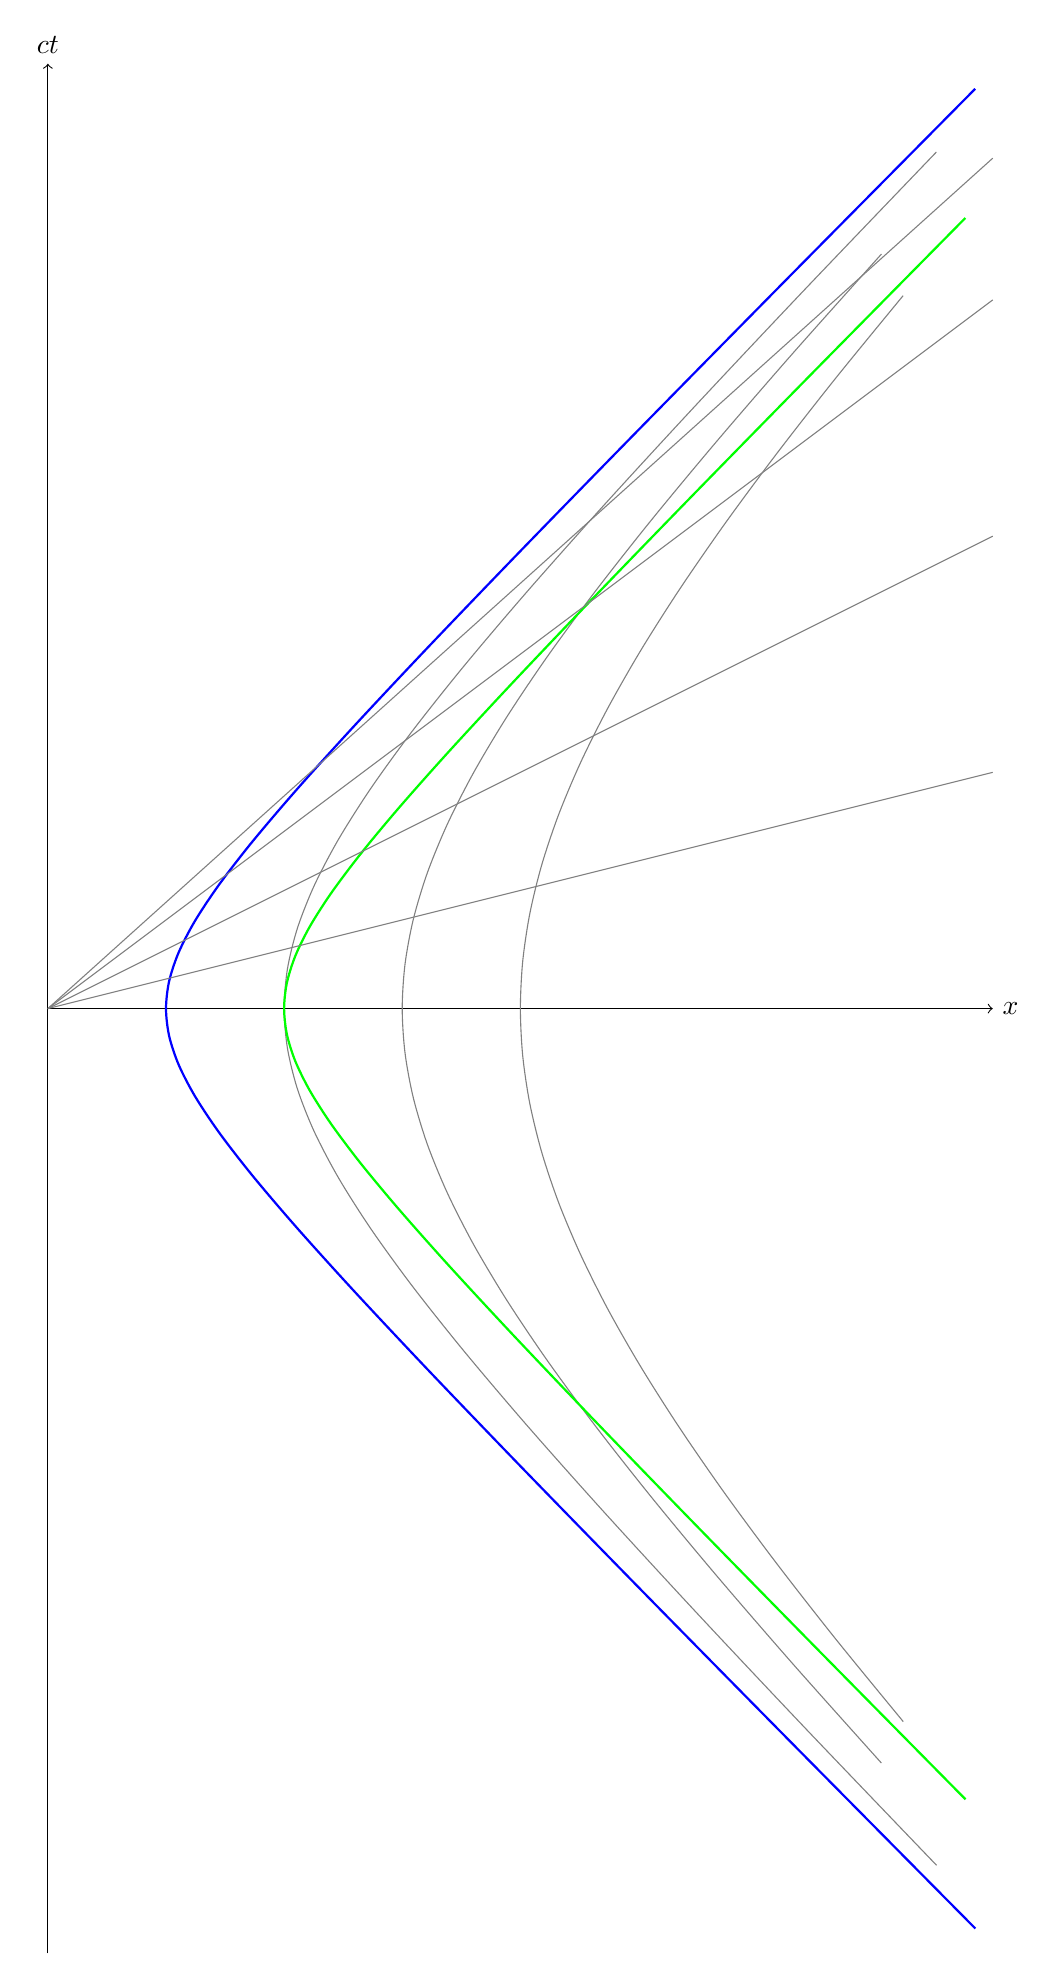
\begin{tikzpicture}[scale=1.5]

    % Draw axes
    \draw[->] (0,0) -- (8,0) node[right] {$x$};
    \draw[->] (0,-8) -- (0,8) node[above] {$ct$};

    % Draw hyperbolic curves (Rindler observers' worldlines)
          \draw[blue,thick,domain=-2.75:2.75, smooth, variable=\y] plot ({cosh(\y)}, {sinh(\y)});        

          \draw[gray,domain=-2:2, smooth, variable=\y] plot ({2*cosh(\y)}, {2*sinh(\y)});

          \draw[gray,domain=-1.5:1.5, smooth, variable=\y] plot ({3*cosh(\y)}, {3*sinh(\y)});

         \draw[gray,domain=-1.2:1.2, smooth, variable=\y] plot ({4*cosh(\y)}, {4*sinh(\y)}); 

         \draw[green,thick,domain=-2.6:2.6, smooth, variable=\y] plot ({1+cosh(\y)}, {sinh(\y)});    

      \draw[gray] plot[domain=0:8] (\x, {0.5*\x}) node[anchor=south west] {};

            \draw[gray] plot[domain=0:8] (\x, {0.25*\x}) node[anchor=south west] {};

            \draw[gray] plot[domain=0:8] (\x, {0.75*\x}) node[anchor=south west] {};

                \draw[gray] plot[domain=0:8] (\x, {0.9*\x}) node[anchor=south west] {};        



  

\end{tikzpicture}
\end{document}



%%% Local Variables:
%%% mode: latex
%%% TeX-master: t
%%% End:
